\documentclass[12pt]{article}
\usepackage{hyperref}
\usepackage{listings}
\usepackage[margin=1in]{geometry}
\usepackage{enumitem}
\usepackage{multicol}
\usepackage{array}
\usepackage{titlesec}
\usepackage{helvet}
\renewcommand{\familydefault}{\sfdefault}
\usepackage{amsmath}     % For math equations
\usepackage{amssymb}     % For advanced math symbols
\usepackage{amsfonts} % For math fonts
\usepackage{gvv}
\usepackage{esint}
\usepackage[utf8]{inputenc}
\usepackage{graphicx}
\usepackage{pgfplots}
\pgfplotsset{compat=1.18}
\titleformat{\section}{\bfseries\large}{\thesection.}{1em}{}
\setlength{\parindent}{0pt}
\setlength{\parskip}{6pt}
\usepackage{multirow}
\usepackage{float}
\usepackage{caption}


\begin{document}
\section*{Problem 4.8.28}

Find the equation of the plane passing through the intersection of the planes
\begin{align}
\vec{r}\cdot(\hat{\imath}+\hat{\jmath}+\hat{k}) &= 1, \\[4pt]
\vec{r}\cdot(2\hat{\imath}+3\hat{\jmath}-\hat{k}) + 4 &= 0,
\end{align}
which is parallel to the $X$--axis. Hence, find the distance of the plane from the $X$--axis.

---

\section*{Input Data}

\begin{table}[H]
\centering
\begin{tabular}{|c |c|}
\hline
Quantity & Value \\
\hline
Normal of $\Pi_1$ & $\vec{n}_1=\myvec{1\\1\\1}$ \\
\hline
Right-hand side of $\Pi_1$ & $b_1=1$ \\
\hline
Normal of $\Pi_2$ & $\vec{n}_2=\myvec{2\\3\\-1}$ \\
\hline
Right-hand side of $\Pi_2$ & $b_2=-4$ \\
\hline
$X$--axis direction & $\vec{e}_1=\myvec{1\\0\\0}$ \\
\hline
\end{tabular}
\caption{Input values for the problem}
\end{table}

---

\section*{Solution}

We first find the line of intersection of the given planes.  
Stacking the two plane equations in matrix form gives
\begin{align}
\vec{A}\vec{r} &= \vec{b}, \\
\vec{A} &= \myvec{\vec{n}_1^\top \\[4pt] \vec{n}_2^\top}
= \myvec{1 & 1 & 1 \\[4pt] 2 & 3 & -1}, \\
\vec{b} &= \myvec{1\\[4pt]-4}.
\end{align}

The augmented matrix is reduced as follows:
\begin{align}
\myvec{1 & 1 & 1 & |&1 \\[4pt] 2 & 3 & -1 & |&-4}
&\xrightarrow{R_2\leftarrow R_2-2R_1}
\myvec{1 & 1 & 1 & |&1 \\[4pt] 0 & 1 & -3 & |&-6} \\[8pt]
&\xrightarrow{R_1\leftarrow R_1-R_2}
\myvec{1 & 0 & 4 & |&7 \\[4pt] 0 & 1 & -3 & |&-6}.
\end{align}

Thus the line of intersection can be expressed as
\begin{align}
\vec{r} &= \vec{r}_p + t\,\vec{d}, \\
\vec{r}_p &= \myvec{7\\[4pt]-6\\[4pt]0}, \\
\vec{d} &= \myvec{-4\\[4pt]3\\[4pt]1}.
\end{align}

Next, since the required plane is parallel to the $X$--axis, its normal $\vec{n}$ must be orthogonal to $\vec{e}_1$.  
Also, since the plane contains the intersection line, $\vec{n}$ must be orthogonal to $\vec{d}$.  
Hence the system is
\begin{align}
\vec{e}_1^\top \vec{n} &= 0, \\
\vec{d}^\top \vec{n} &= 0.
\end{align}

Writing this in matrix form:
\begin{align}
\myvec{\vec{e}_1^\top \\[4pt] \vec{d}^\top}\vec{n}
&= \myvec{1 & 0 & 0 \\[4pt]-4 & 3 & 1}\vec{n}
= \myvec{0\\0}.
\end{align}

The augmented matrix reduces as
\begin{align}
\myvec{1 & 0 & 0 & |&0 \\[4pt]-4 & 3 & 1 & |&0}
&\xrightarrow{R_2\leftarrow R_2+4R_1}
\myvec{1 & 0 & 0 & |&0 \\[4pt]0 & 3 & 1 & |&0}.
\end{align}

From this we conclude
\begin{align}
n_x &= 0, \\
3n_y + n_z &= 0.
\end{align}

Choosing a convenient scale, we may take
\begin{align}
\vec{n} &= \myvec{0\\[4pt]-1\\[4pt]3}.
\end{align}

Now the constant term of the plane is obtained by substituting a point $\vec{r}_p$ on the line:
\begin{align}
c &= \vec{n}^\top \vec{r}_p, \\
c &= \myvec{0 & -1 & 3}\myvec{7\\[4pt]-6\\[4pt]0}, \\
c &= 6.
\end{align}

Therefore, the equation of the required plane is
\begin{align}
\vec{n}^\top\vec{r} - c &= 0, \\
\vec{n}^\top\vec{r} - 6 &= 0.
\end{align}

Finally, the distance of this plane from the $X$--axis is
\begin{align}
d &= \frac{|c|}{\|\vec{n}\|}, \\
d &= \frac{6}{\sqrt{\vec{n}^\top\vec{n}}}, \\
d &= \frac{6}{\sqrt{10}}.
\end{align}

---

\section*{Final Answer}

\begin{align}
\boxed{\;\vec{n}^\top\vec{r} - c = 0\;}, \qquad
\boxed{\;\vec{n} = \myvec{0\\[4pt]-1\\[4pt]3}, \; c = 6\;}, \qquad
\boxed{\;\mathrm{distance} = \tfrac{6}{\sqrt{10}}\; }.
\end{align}

\begin{figure}[H]
    \centering
    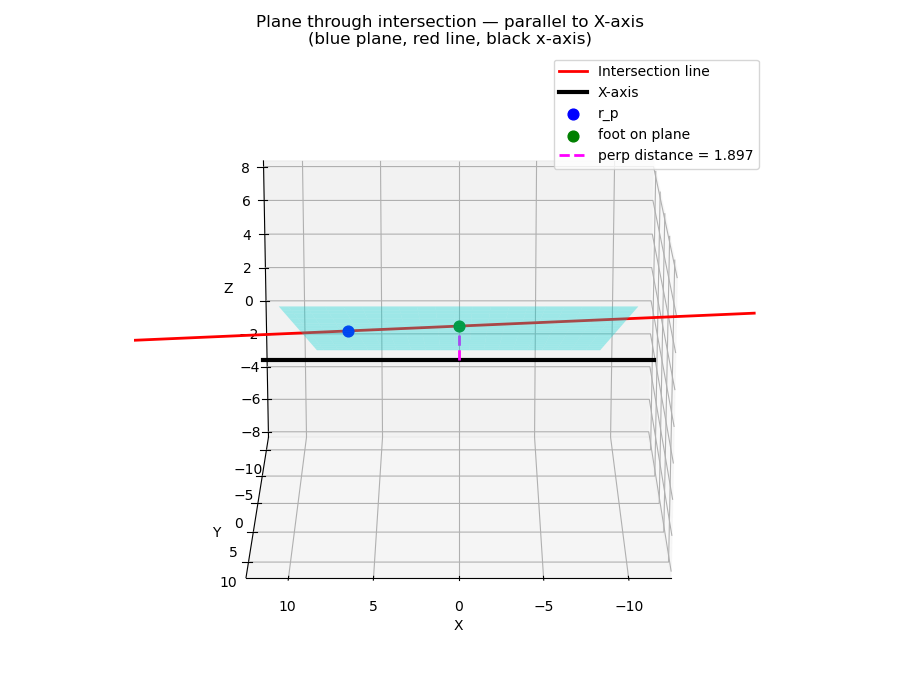
\includegraphics[width=0.9\columnwidth]{figs/new_plane.png}
    \caption{}
    \label{fig:placeholder}
\end{figure}


\end{document}
